\chapter{Object Reconstruction and Selection}
\label{sec:obj_reconstruction}

In this chapter I discuss the progression from detector-based signals through to an
overall event reconstruction within CMS. At CMS, physics-object reconstruction draws
on input from all detector subseystems simultaneously to build particle tracks
and cluster together energy deposits, to link together these tracks and energy
deposits to construct basic physics-objects such as electrons and charged
hadrons, and to build composit objects such as ``jets'' and hadronically decaying
$\tau$ leptons. Event based quantities such as the \etvecmiss are also reconstructed.
To achieve all of this, CMS uses its Particle Flow (PF) reconstruction 
algorithm~\cite{Sirunyan:2017ulk}. The particle flow concept has been used in the 
past by other experiments such as ALEPH at LEP~\cite{PF-ALEPH}. CMS is the first
experiment to fully utilize the particle flow techinque in a hadron collider environment.
A discussion of the reconstruction of the two elemental PF objects, tracks and energy
clusters, follows in the next section. Afterwards I detail the construction of 
the PF physics-objects then move to composit objects and full event variables.
The PF approach allows particles from pileup interactions to be identified 
and enables efficient pileup mitigation methods.

\section{Particle Flow Input}
The CMS detector and the PF reconstruction algorithm were specifically designed to
compliment eachother. The CMS detector features: a highly-segmented tracker well
suited to precise track reconstruction, a fine-grained electromagnetic calorimeter necessary
to separate the individual energy deposits from particles within ``jets'' and
for efficient photon and electron identification, a hermetic hadron 
calorimeter for the measurement and identification of charged and neutral hadrons, 
a strong magnetic field for the measurement of the momenta of charged particles and to
separate the calorimeter energy deposits of charged and neutral hadrons within ``jets'', and 
an excellent muon spectrometer for muon identification and to disintangle the muon
tracks from other tracks in the tracker. A schematic of a slice of the CMS detector
and different physics-objects transversing the detector subsystems can be see in
Figure~\ref{fig:cms_slice}. The different detector systems all contribute
necessary pieces of information to the PF reconstruction. From the raw detector
signals two classes of PF objects are created, tracks and energy clusters.

\begin{figure*}[htbp]
\centering
     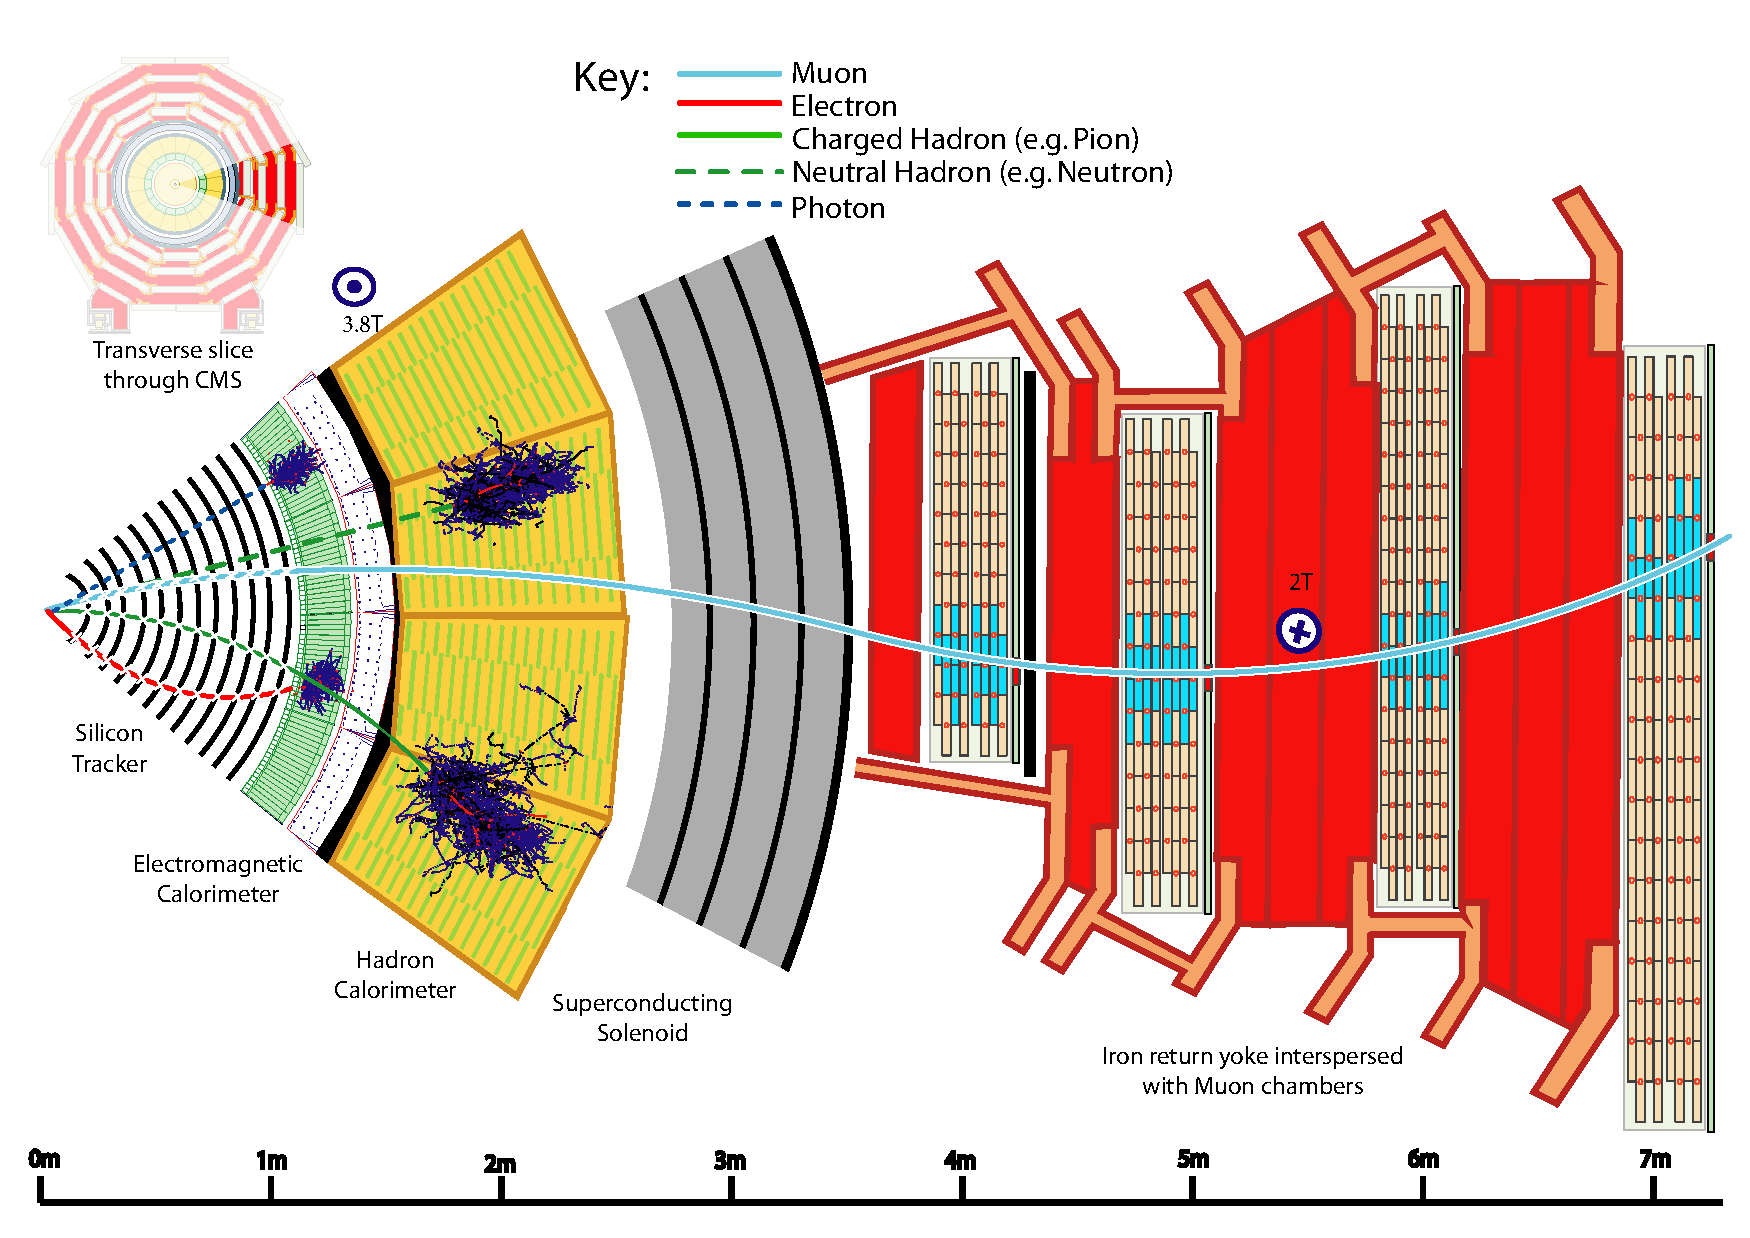
\includegraphics[width=1.0\textwidth]{object_reconstruction_and_selection/plots/cms_slice.pdf}
     \caption{
A schematic of a slice of an x-y cross section of the CMS detector showing different
physics-objects such as electrons, photons, charged and neutral hadrons, and muons
propagating outwards from the collision region within the detector. The schematic
shows how tracks are linked to energy deposits and in which subdetectors different
particles deposit most of their energy on average.
     }
     \label{fig:cms_slice}
\end{figure*}


\subsection{Particle Flow Tracks}
\label{sec:pf_tracks}
Energy deposits, often called ``hits'', are recorded by the pixel and strip tracker during
a collision. From these, charged particle tracks are reconstructed in subsequent layers
mapping the progression of charged particles from the beam axis outwards into the detector
volume. Attempting to reconstruct tracks from every possible hit combination quickly
because unreasonable considering the over 70 million tracker pixels and strips which can
each record a hit. PF uses a combinatorial track finder based on Kalman 
Filtering (KF); the algorithim is broken down into three successive steps.
\begin{itemize}
\item Generate seed tracks from a few hits which are compatible with a charged
particle trajectory
\item Gathering other hits along the seed track trajectory when propagated through
the rest of the tracker subsystem
\item Final track fitting to determine track properties such as the origin, transverse
momentum, and direction.
\end{itemize}
Only tracks meeting certain quality standards are kept for analysis. These tracks must
be seeded with two hits in consecutive layers in the pixel detector, and are required 
to be reconstructed with at least eight tracker hits in total, and with at most one 
missing hit along the track trajectory. Tracks must also have a curvature corresponding
to a momentum greater than 0.9\GeV.

There is a balance that must be struck between imposing tight quality cuts on reconstructed
tracks, which increases the purity of genuine track within the reconstructed track collection,
but also decreases the efficiency for reconstructing genuine tracks, and loosening
quality cuts to reconstruct genuine tracks with a higher efficiency and lower purity.
After an initial pass through what is called the global combinatorial track finder,
which has the stringent track quality criteria impossed by the eight hit requirement
mentioned above, the efficiency to reconstruct
genuine tracks is roughly 80\% for charged pions with $\pt = 10\GeV$, and 99\%
for isolated muons. This corresponds to a misreconstructed track rate of
about 2.5\% for charged pions with $\pt = 10\GeV$, see Figure~\ref{fig:kf_tracking}.
As hits are recorded in a reconstructed track, they are removed from the available,
unused hits which can be combined in subsequent passes through the tracking algorithm.

There are ten passes through the tracking algorithm in total. Each pass loosens the track quality criteria,
such as $\chi^2$ and number of hits requirements, beyond the stingent initial criteria.
This helps to reconstruct difficult to build tracks. Tracks can be difficult to 
reconstruct for multiple reasons such as detector inefficiencies leading to missing
detector hits, or particles originating from elsewhere in the detector 
besides along the beam axis. These tracks could be from hadrons interacting
within the tracker material before reaching the eight-hits threshold, or from the decay
of particles with finite life-times. Additionally, there can be difficulty disintangling
the many tracks within a collimated ``jet'' where many of the tracks are close to or
nearly overlapping with one another.
The misreconstruction rate is suppressed in each iterative step despite the loosening
quality criteria by the removal of the hits which are previously incorporated into
a reconstructed track. This  suppresses the random hit-to-seed association in the
next iteration and allows moderate efficiency gains for only small misreconstruction losses.
The efficiency and misreconstruction rate in Figure~\ref{fig:kf_tracking} shows the
results for i) the initial pass through the tracking algorithm, ii) the results after all
passes which require the track seed to contain hits in the pixel detector, and iii) the
final results after considering displaced tracks.
After all iterations the efficiency is about 90\% for a charged pions with $\pt = 10\GeV$
for a misreconstruction rate of 3\%.

\begin{figure*}[htbp]
\centering
     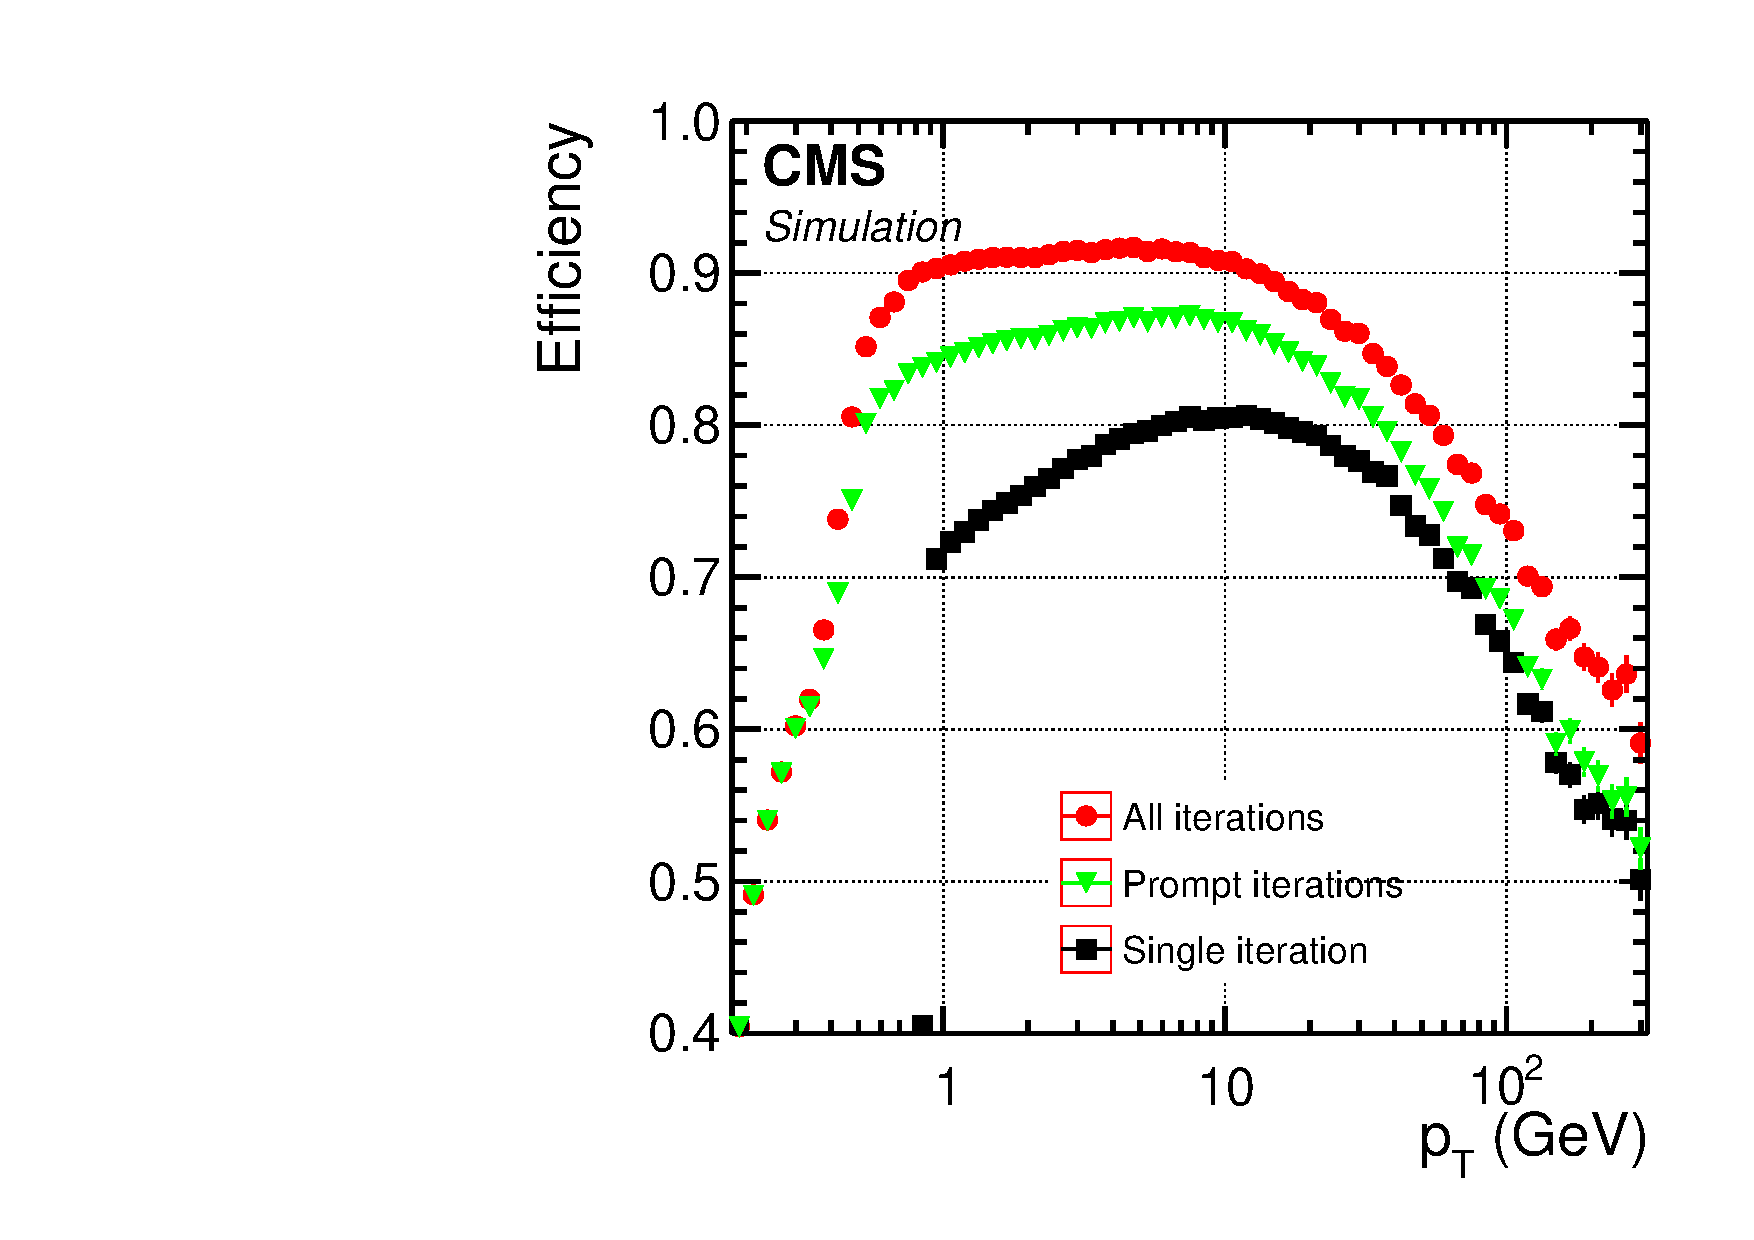
\includegraphics[width=0.45\textwidth]{object_reconstruction_and_selection/plots/pf_track_eff.pdf}
     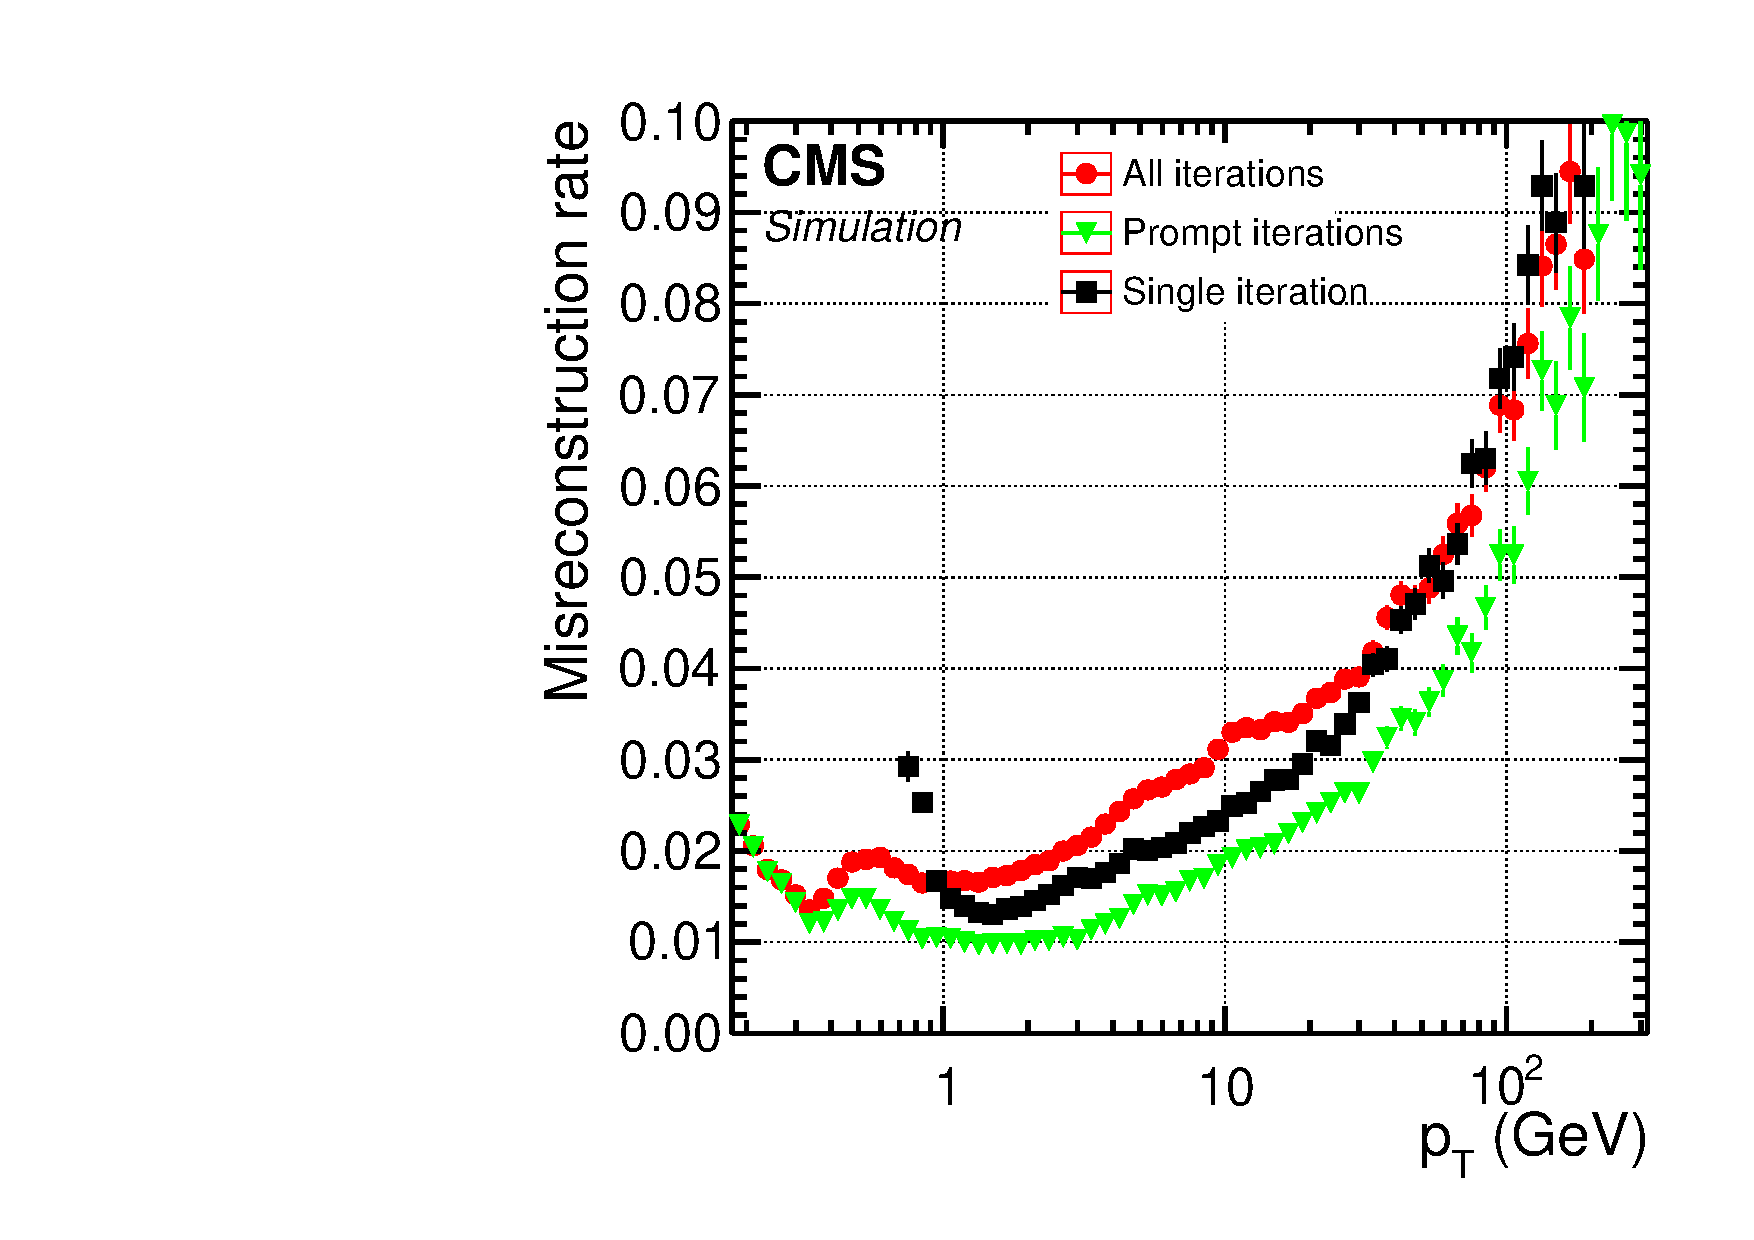
\includegraphics[width=0.45\textwidth]{object_reconstruction_and_selection/plots/pf_track_misId.pdf}
     \caption{
Efficiency (left) and misreconstruction rate (right) of the global combinatorial track finder (black squares) 
which is the first pass through the tracking algorithm. The prompt iterations of the tracking method (green 
triangles) show the results after all iterations based on seeds with at least one 
hit in the pixel detector are completed. The final results after all iterations (red circles) includes
iterations with displaced seeds. Efficiency and misreconstruction rate are plotted as a function 
of the track $\pt$, for charged hadrons in multijet events without pileup interactions. Only tracks with 
$\abs\eta < 2.5$ are considered. The efficiency 
is displayed for tracks originating from within 3.5 cm of the beam axis and $\pm$30 cm of the nominal 
centre of CMS along the beam axis.
     }
     \label{fig:kf_tracking}
\end{figure*}

Tracks which are likely associated with electrons receive special treatment in PF. Electrons
will often emit bremsstrahlung radiation while propagating through the tracker.
When energetic photons are radiated from an electron, the pattern recognition in the KF algorithm
may have difficulty accommodating the sudden change in electron momentum. This can cause the track to 
be reconstructed with a smaller number of hits than would be associated with the true electron
path. A new collection of tracks is created based on a preselection on the number of hits and 
the $\chi^2$ for the reconstructed KF-based tracks. The new collection which is a subset of the
KF-based tracks are fit again with a Gaussian-sum filter (GSF)~\cite{gsf_electrons}. Instead of
modeling the energy loss of particles as a single gaussian probability density function (PDF) like the KF
algorithm does, the GSF models the energy loss as a mixture of multiple gaussian PDFs. 
The GSF fitting algorithm is more adapted to electrons than the KF algorithm.
It allows for sudden and substantial energy losses along the trajectory. The
additional freedom here allows much better fits for the electron-based tracks and provides
better estimates for the track origin, trajector towards the calorimeters, and $\pt$.

Muon tracks are built from a combination of the pixel and strip tracker (inner tracker) information and the
muon spectrometer information. 
The hits in the muon spectrometer are quite pure in genuine muon hits. This is because of the
calorimeters and the solenoid which absorb the vast majority of non-muon particles, except neutrinos, 
before they reach the muon spectrometer. There are three different categories of muon tracks
reconstructed:
\begin{itemize}
\item Standalone muons are based on hits within each DT or CSC detector. Hits are clustered to form 
track segments that are used as seeds for the pattern recognition in the muon spectrometer to gather
other hits in the muon systems along the track trajectory.
\item Global muons are reconstructed from a standalone-muon track which is matched to a track 
from the inner tracker. If the trajectories of the two tracks propagate onto a common surface 
they are considered compatible and the hits from the inner tracker and from the standalone-muon 
track are combined and fit to form a global-muon track.
\item Tracker muons are built from an extrapolation of a track from the inner track system to a
single compatibe muon segment within the muon spectrometer system. The inner tracker-based track must have 
a $\pt > 0.5\GeV$ and a total momentum $p > 2.5\GeV$.
\end{itemize}

About 99\% of the muons produced within the geometrical acceptance of the muon system are 
reconstructed either as a global muon or a tracker muon and very often as both.
For muons with $\pt > 200\GeV$, the momentum resolution, based on the inner track, is 
improved by the inclusion of the track extension to the muon system.
For muons with $\pt < 200\GeV$, the inner tracker already provides a precise measurement of 
their momentum.


\subsection{Particle Flow Energy Clusters}
Energy clusters make up the second basic PF building block. The PF energy
clustering algorithm used to constructs the energy clusters serves multiple purposes:
\begin{itemize}
\item Detect and measure the energy and direction of stable neutral particles (photons and neutral hadrons)
\item Separate neutral particles from charged hadron energy deposits
\item Reconstruct and identify electrons and all accompanying bremsstrahlung photons
\item Assist the energy measurement of charged hadrons for which the track parameters were not 
determined accurately; this is primairly the case for low-quality and high-$\pt$ tracks
\end{itemize}
The clustering is performed separately in each subdetector, the ECAL barrel and endcaps and HCAL barrel
and endcaps with an aim of a high detection efficiency even for low-energy particles and the ability to 
separat close energy deposits. Clustering begins with seed hits which have an energy above the seed hit
threshold and an energy larger than the energy of the adjacent hits. The fine granularity of the 
ECAL barrel allows
for the clustering to consider all eight adjacent hits, four on the sides and four on the corners.
The HCAL barrel has a more coarse granularity. Only the four adjacent sides are considered when
selecting a seed candidate. From the starting seed, topological clusters are grown outward by aggregating
hits with at least a corner in common with a cell already included in the cluster. Hits must have an energy
in excess of two times the subdetector noise level to be considered for clustering. The energy thresholds
for seeding a cluster and cluster inclusion threshold are in Table~\ref{tab:pf_cluster_thresholds}.


\begin{table*}[htbp]
\centering
\begin{footnotesize}
%\begin{scriptsize}
\begin{tabular}{|l|cc|cc|}
\hline
        &       \multicolumn{2}{|c|}{ECAL}        &       \multicolumn{2}{|c|}{HCAL}        \\  %&   Preshower \\
        &   barrel  &   endcaps        &       barrel   &   endcaps        \\  %&    \\
\hline
Cell $E$ threshold (\MeV) & 80 & 300    &   800 &   800 \\   %& 0.06 \\
\hline
Seed Number closest cells   &   8 & 8   &   4 & 4 \\    %& 8 \\
Seed $E$ threshold (\MeV)   &  230  &  600  &  800  & 1100 \\    %& 0.12  \\
Seed $E_{\text{T}}$ threshold (\MeV)   &  0  &  150  & 0   & 0 \\    %& 0 \\
%\hline
%Gaussian width (cm)   &  1.5  &  1.5  &  10.0  & 10.0  \\    %& 0.2 \\
\hline
\end{tabular}
\end{footnotesize}
%\end{scriptsize}
\caption{
The clustering parameters used for ECAL and HCAL energy deposit clustering. The ECAL endcap
requires an additional seed $E_{\text{T}}$ threshold because the detector noise
increases as a function of $\abs\eta$.
}
\label{tab:pf_cluster_thresholds}
\end{table*}

Residual energy calibrations are applied to the ECAL and HCAL energy clusters. The calibrations are
designed to account for the effects of the hit energy thresholds which will always result in a 
smaller amount of energy being incorporated into a cluster than was measured by the detector
for a given single object.
In the ECAL, the residual energy calibration is determined from simulated single photon events.
This generic calibration is applied to all ECAL clusters prior to the hadron cluster calibration 
mentioned next. 

ECAL and HCAL energy clusters are linked together as a potential hadronicy decay energy deposit
if their positions in \etaphi overlap. For a hadronic decay, the total calorimeter response (ECAL + HCAL) depends on 
the fraction of the shower energy deposited in the ECAL, and is not linear with energy. The 
ECAL and HCAL cluster energies are calibrated to get an 
estimate of the true hadron energy. Simulated single neutral hadrons, specifically 
$\text{K}^{0}_{\text{L}}$s, are used for the hadronic decay response calibration seen
in Figure~\ref{fig:pf_calo_calib}. The applied calibrations in the left plot lead
to excellent agreement in the calorimeter response in the right plot.

\begin{figure*}[htbp]
\centering
     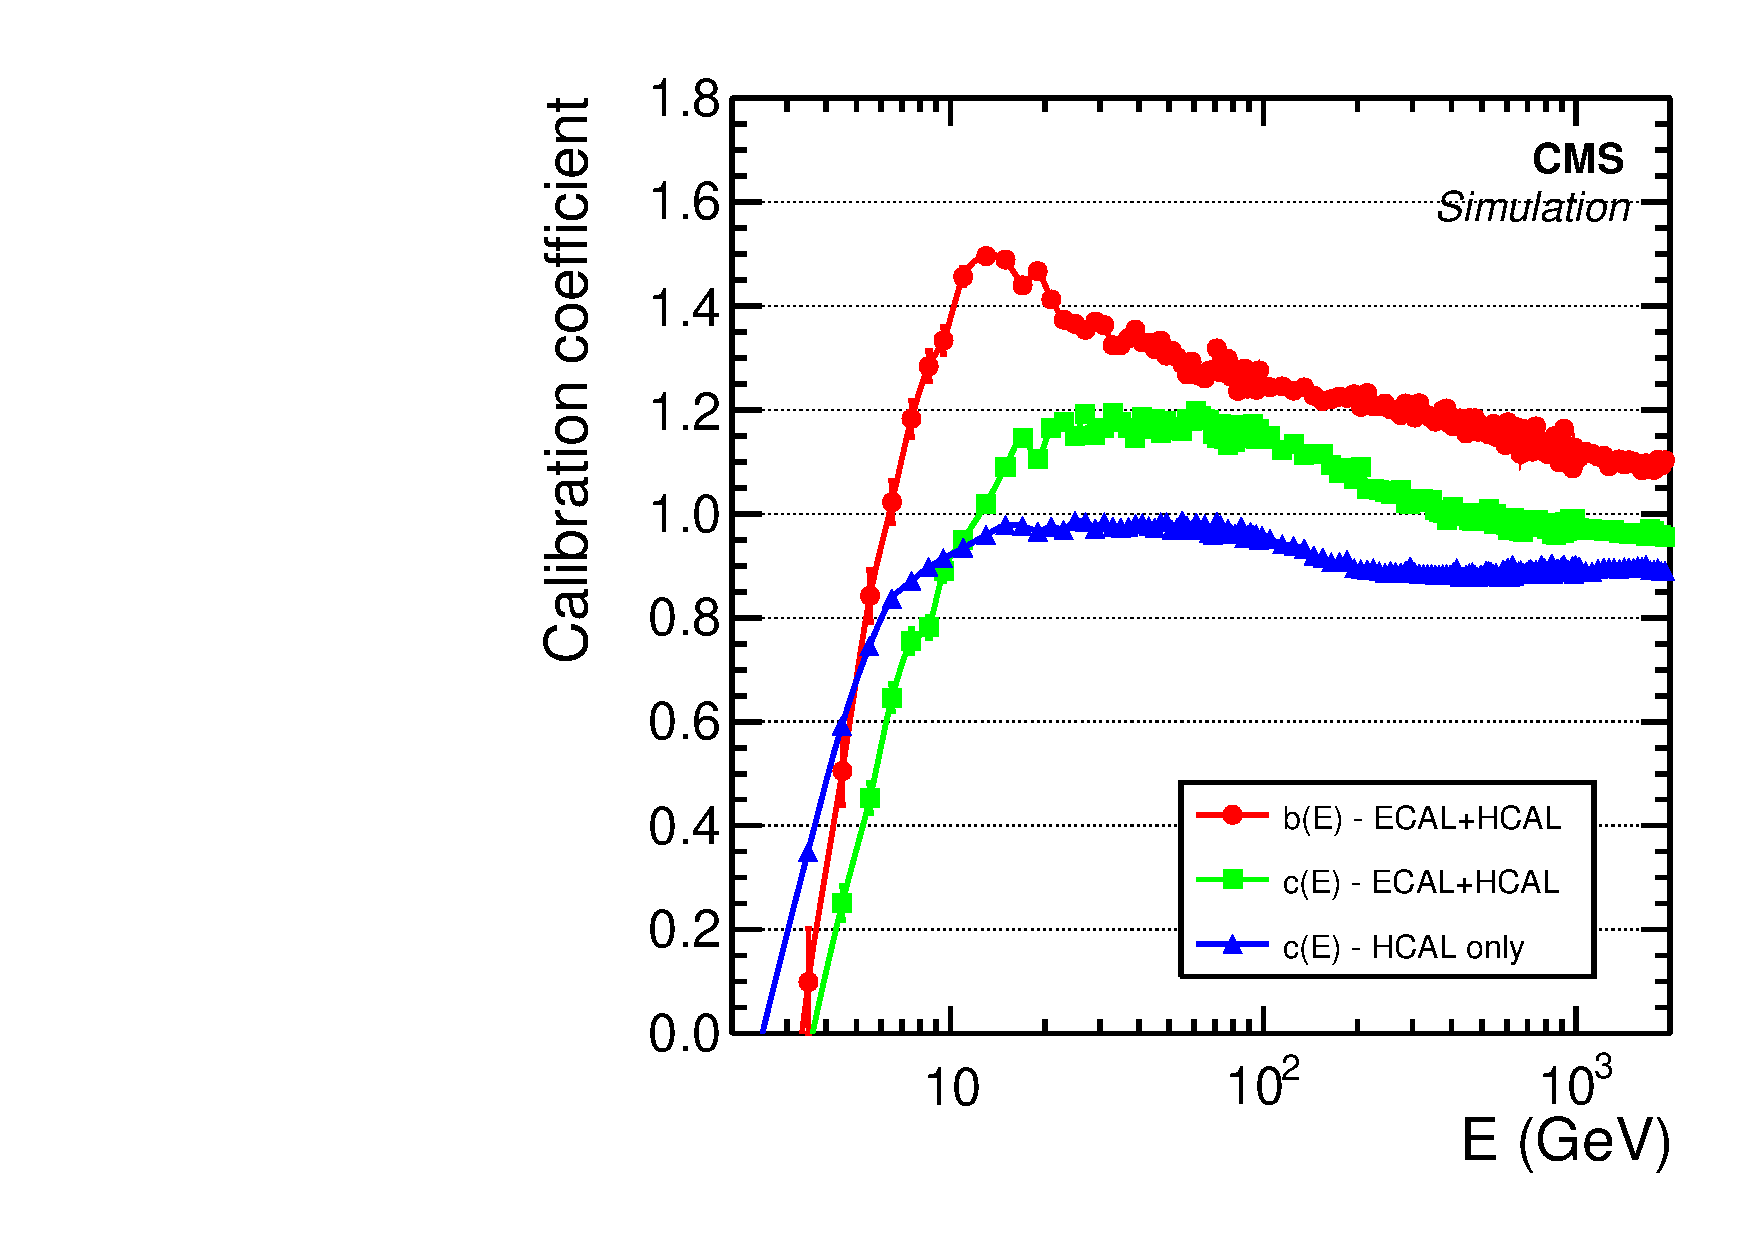
\includegraphics[width=0.45\textwidth]{object_reconstruction_and_selection/plots/calo_calibrations.pdf}
     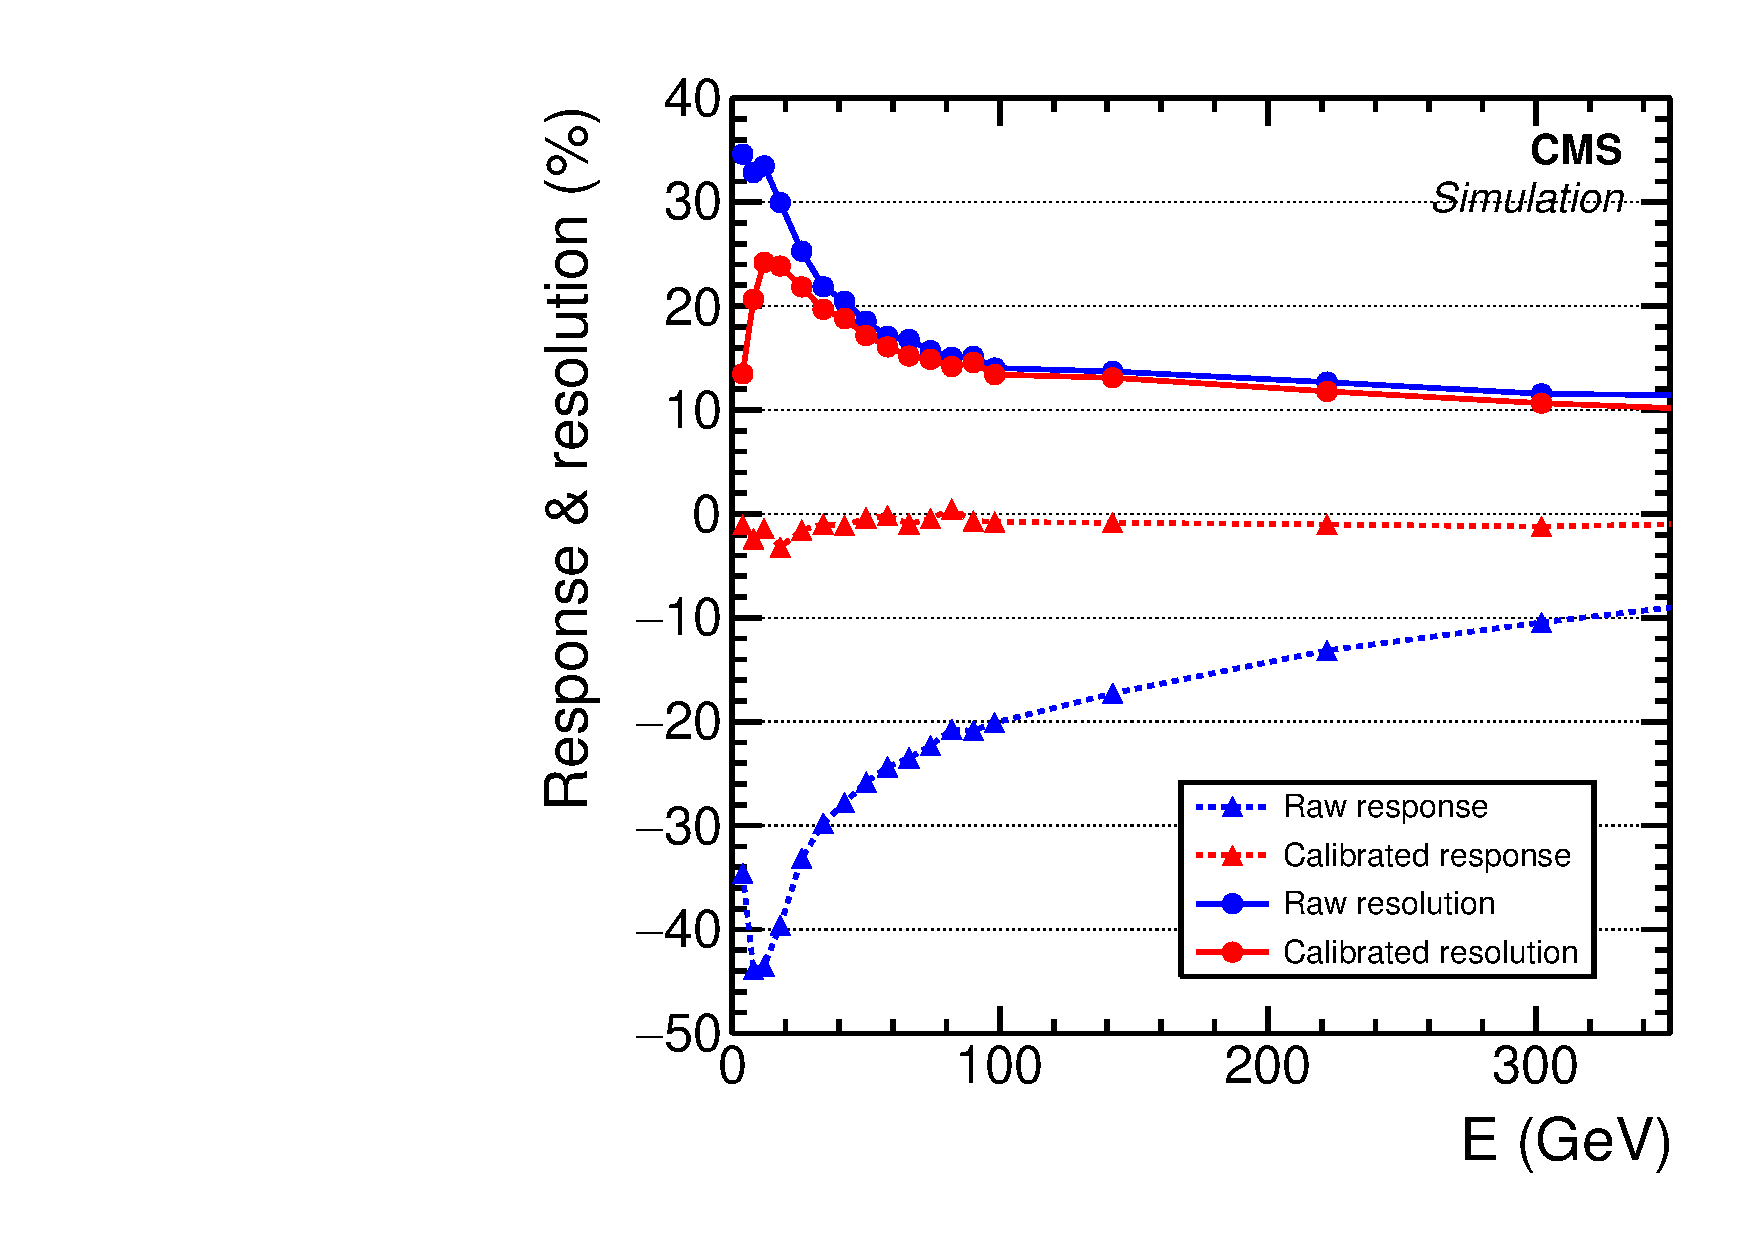
\includegraphics[width=0.45\textwidth]{object_reconstruction_and_selection/plots/calo_response_and_res.pdf}
     \caption{
(left) Calibration coefficients obtained from single $\text{K}^{0}_{\text{L}}$s in the barrel as a 
function of their true energy $E$. The blue triangles show the calibrations for hadrons depositing 
energy only in the HCAL. The red circles (green squares) show the ECAL (HCAL) calibration for hadrons
depositing energy in both the ECAL and HCAL.
(right) Relative energy response (dashed curves) for the raw (blue) and calibrated (red) energy, and 
energy resolution (solid curves). Both for single $\text{K}^{0}_{\text{L}}$s in the barrel as a 
function of their true energy $E$.
%Here the raw (calibrated) response and resolution are obtained by a Gaussian fit to the distribution of 
%the relative difference between the raw (calibrated) calorimetric energy and the true hadron energy.
     }
     \label{fig:pf_calo_calib}
\end{figure*}


In general, a given particle (physics-object) propagating through the CMS detectoris 
is expected to result in multiple PF elements (tracks and energy
clusters) in various CMS subdetectors. The reconstruction of a particle begins 
with a linking algorithm that connects the PF elements from different subdetectors. For example,
tracks are linked to energy clusters if the extrapolated trajectory of the track aligns within the
angular acceptance of an energy cluster in \etaphi. Energy clusters can be linked between subdetectors as mentioned
in the case of hadronic energy deposits above which can span both the ECAL and HCAL. A link is established
when the cluster position in the more granular calorimter (ECAL) is within the cluster envelope
in the less granular calorimeter (HCAL). Once PF elements are linked together they are referred to as a PF block which can contain 
elements associated either by a direct link or by an indirect link through common elements.


\subsection{Particle Flow Candidates}
Particle Flow candidates are selected from the PF blocks based on compatibility with
different physics-object characteristics and designated quality cuts.


\subsubsection{Muons}
Isolated global muons are selected from the global muon track colletion by looking at the inner
tracker tracks and calorimeter 
energy deposits within a distance $\dr < 0.3$ to the muon trajectory. 
The sum of the $\pt$ of the tracks and of the $E_{\text{T}}$ of the energy deposits is required not to 
exceed 10\% of the muon $\pt$. This isolation criterion alone successfully reject hadrons that would
otherwise be misidentified as muons. No further selection is applied to these muon candidates.
If the muon track $\pt < 200\GeV$, then the momentum assigned to the muon PF candidate is that of 
the inner track. For muon tracks with $\pt > 200\GeV$, the momentum assigned is the momentum associated
with the smallest $\chi^2$ probability from these different track fits: tracker only, tracker and 
first muon detector plane, global, and global without the muon detector planes featuring a high occupancy.
The PF elements and blocks that make up an identified PF muon candidate are masked against further processing
to prevent their inclusion in other PF candidates.

In these analyses, there are several additional criteria applied beyond 
being a basic PF muon candidate. These analyses use muons which pass two different PF muon identification working
points: \texttt{PF ID Loose} and \texttt{PF ID Medium}~\cite{sm-htt-2017}. The \texttt{PF ID Loose}
working point is only slightly tighter than the baseline criteria for a PF muon candidate; 
a \texttt{PF ID Loose} muon must be either a global or a tracker PF muon. This selection is highly efficient
for prompt muons.

The \texttt{PF ID Medium} muon working point requires first that muons pass \texttt{PF ID Loose} then
applies additional track-quality and muon-quality requirements on the different muon tracks which are
linked to the PF muon candidate. The number of valide inner tracker
hits must be greater than 80\%. Additionally, either one of the following criteria must be met:
\begin{outline}
\1 Option 1 - ``Tight Segment Compatility''
    \2 Candidate has a segment compatility score of at least 0.451 which ensures that the 
track is reasonablly compatible with inner tracker-based track
\1 Option 2 - ``Good Global Muon'':
    \2 PF muon candidate is a global muon
    \2 The normalized track $\chi^2 < 3$
    \2 The compatibility $\chi^2$ between the standalone muon track and the inner tracker muon is
less than 12
    \2 The muon track kink-finder, which is desiged to remove muons produced from in-flight decays, 
must have a value less than 20
    \2 Candidate has a segment compatility score of at least 0.303 which is looser than the value
required in Option 1
\end{outline}
The \texttt{PF ID Medium} muon working is still very efficienct for prompt muon selection but
does bring some additional reduction in fake object selection which is helpful in the high
statistics $\htt$ analysis. 

To reject non-prompt or misidentified muons and electrons, a relative lepton isolation is defined as:
\begin{equation}
I^{\ell} \equiv \frac{\sum_{charged}  \pt + \max\left( 0, \sum_{neutral}  \pt
                                         - \frac{1}{2} \sum_{charged, PU} \pt  \right )}{\pt^{\ell}}.
\label{eq:rel_isolation}
\end{equation}

Some of the quantities mentioned here refer to descriptions in the following sections.
In this expression, $\sum_{charged}  \pt$ is the scalar sum of the transverse energy of the 
charged particles originating from the primary vertex and located in a cone of size
$\dr = \sqrt{\smash[b]{(\Delta \eta)^2 + (\Delta \phi)^2}} = 0.4$\,(0.3)
centered on the muon (electron) direction. The sum, $\sum_{neutral}  \pt$, represents
a similar quantity for neutral particles. The contribution of photons and neutral hadrons 
originating from pileup vertices is estimated from the scalar sum of the transverse
energy of charged hadrons in the cone originating from pileup vertices,
$\sum_{charged, PU} \pt$. This sum is multiplied by a factor of $1/2$, which corresponds 
approximately to the ratio of neutral to charged hadron production in the hadronization process
of inelastic $\Pp\Pp$ collisions, as estimated from simulation. The expression $\pt^{\ell}$ 
stands for the $\pt$ of the lepton. Isolation requirements used in the following analyses
for electrons and muons range from $I^{\ell} < 0.1$ to $I^{\ell} < 0.25$ depending on the signal efficiency and
background rejection needs of the specific final state. For the $\htt$ analysis, these
working points are listed in the $\htt$ analysis section, Table~\ref{tab:htt_obj_selection}.


\subsubsection{Electrons and Prompt Photons}
With the muon related PF elements masked from further processing, electron and prompt photon
identification begins.
Electron identification is based on information from the inner tracker tracks and the calorimeter
energy clusters. Because of bremsstrahlung radiation, electron tracks can be much more kinked
than those for other particles as was discussed above in relation to the GSF algorithm track
fitting. Additionally, because of radiated bremsstrahlung photons, the resulting energy clusters 
from an electron propagating through the detector can be spread out in the
$\phi$ direction. PF electrons are built from the linking of a GSF track to an
ECAL-based energy cluster. To suppress the amount of charged hadrons faking electrons, the 
sum of the energies measured in HCAL hits behind ($\dr < 0.15$) 
the electron-linked ECAL energy cluster must no exceed 10\% of the ECAL-based 
energy cluster energy~\cite{Sirunyan:2017ulk}. The energy assignment for an electron candidate is obtained from a 
combination of the calibrated ECAL energy with the momentum of the GSF track. The electron 
direction is chosen to be that of the GSF track.

Before being saved to the PF electron collection, electron candidates must satisfy additional
identification criteria targeted at reducing electron fakes. Up to fourteen variables are
fed into a Boosted Decision Tree (BDT) which determines the passing PF electrons. The BDT
input variables include track and energy cluster details such as:
\begin{itemize}
\item Amount of energy radiated off the GSF track
\item Distance between the GSF track extrapolation to the ECAL entrance and the position of the ECAL cluster
\item Ratio between the HCAL and ECAL energies
\item The KF and GSF track $\chi^2$ values, and
\item The numbers of inner tracker hits
\end{itemize}

Photon candidates are seeded by ECAL energy clusters with no matching KF or GSF track.
They are retained as PF photons if they are isolated from other tracks and calorimeter energy clusters, 
and if the ECAL energy distribution and the ratio between the HCAL and ECAL energies, $H/E$, are 
compatible with those expected from a photon shower. Similar to the PF masking after the muon 
reconstruction, tracks and energy clusteres used to
build PF electron and photons are masked from further processing simplifying the task ahead
for charged and neutral hadron identification.

There are additional electron identification requirements used in these analyses which are tighter
than the PF electron criteria. The additional identification criteria relies on a multivariate (MVA) discriminant
which combines many of the same variables used in the PF electron BDT~\cite{Khachatryan:2015hwa} 
and addes some additional energy cluster distribution variables such as $\sigma_{i\eta i\eta}$ and
$\sigma_{i\phi i\phi}$ cluster shape covariance. The analyses use
two different MVA working points, one with 90\% signal efficiency and one with 80\% efficiency.


\subsubsection{Charged and Neutral Hadrons}
Once muons, electrons, and isolated photons are identified and removed from the available PF blocks, 
the remaining particles to be identified are hadrons resulting from jet fragmentation and 
hadronization. The ECAL and HCAL energy clusters which are not linked to any tracks are turned into
PF neutral hadrons while energy deposits successfully linked to a track are turned into PF charged
hadrons. Non-isolated photons are indistinguishable from the neutral hadron group.
Charged and neutral hadrons form the last sets of fundamental physics-objects
which are reconstructed by PF. The next PF steps involve reconstructing composit object such as ``jets''
and hadronically decaying tau leptons and calculating event quantities such as the primary vertex and
\etvecmiss.


\section{Event Level Quantities}
There are multiple event level quantities that require input from all PF physics-objects for their
calculation.


\subsection{Primary Vertex Reconstruction}
The original location of the $\pp$ collisions which gave rise to a given event can be found by tracing
the reconstructed physics-object tracks back to the collision region and grouping together tracks that share a common
origin; the origins are called vertices. In any given recorded collision there will usually be a 
singular hard-scatter $\pp$ collision and multiple soft-scatter collsion. The hard-scatter vertex is 
identified as the vertex with the largest quadratic sum of the $\pt$ of the associated physics-objects 
and is called the primary vertex~\cite{Sirunyan:2017ulk}. The other vertices are referred to as the
pileup vertices. The calculation of the primary vertex is specifically needed for the identification of
composit objects such as ``jets'' and hadronically decaying $\tau$ leptons.


\subsection{Missing Transverse Energy}
\label{sec:obj_reco_met}
The CMS detector can detect and measure the energy of all standard model particles with the exception
of neutrinos which leave the detector undetected. The neutrino energy contribution to an event can
be estimated using the missing transverse energy, \etvecmiss. The \etvecmiss is calculated from
the missing transverse momentum vector which is defined 
to balance the vectorial sum of the transverse momentum of all particles.

\begin{equation}
\vec{p}^{\text{miss}}_{\text{T,PF}} = - \sum^{N_{\text{particles}}}_{i=1} \vec{p}_{\text{T},i}
\end{equation}

All particles reconstructed in the event are used to determine the missing transverse energy,
\etvecmiss~\cite{Khachatryan:2014gga}. The specific \etvecmiss used in these analyses is Type-1
\etvecmiss which is adjusted for the effect of jet energy corrections.


\section{Composit Object Identification and Selection}
Composit objects reconstructed by PF cluster together physics-objects which likely
resulted from the jet fragmentation or hadronization process. The three groups used in these
analyses are discussed below.

 
\subsection{Jets}
\label{sec:obj_reco_jets}
Jets are collections of energy deposits and tracks within a defined conical area radiating outward
from the collision region. They are created when a quark or gluon undergoes the hadronization process.
Jets are reconstructed with an anti-\kt clustering algorithm implemented in the \FASTJET 
library~\cite{Cacciari:2008gp, Cacciari:2011ma, Cacciari:fastjet2}. The anti-\kt clustering is based on the grouping
together of neutral and charged PF candidates within a distance parameter $\dr = 0.4$. Charged PF 
candidates not associated with the primary vertex are not considered when building jets.
A correction is applied to jet energies to adjust for the contribution to the jet energy from 
additional $\pp$ interactions within the same or nearby bunch crossings. The energy of a jet is 
corrected via calibrations based on simulation and data~\cite{CMS-JME-10-011}.


\subsection{b-jet Identification}
Jets which result from the decay and hadronization of b quarks are used to help classify events
in the $\htt$ analyses. B quarks are not produced from the four leading Higgs boson production
mechanisms. Therefore, in multiple final states, events with jets which are likely caused by the decay and
hadronization of b quarks are a likely sign of a background event.
The combined secondary vertex (CSVv2) algorithm is used to identify jets that likely resulted
from a b quark decay, a ``b-jet''. The CSVv2 algorithm uses track-based lifetime information together with 
the reconstructed secondary vertices associated with the jet to provide a likelihood ratio 
discriminator for b-jet identification. The b jet identification working point chosen in the $\htt$ analyses 
gives an efficiency for identifying genuine b jets of about 70\%, and for misidentifying light flavor jets
as b jets of about 1\%.


\subsection{Taus}
\label{sec:obj_reco_tau}
Hadronically decaying $\Pgt$ leptons are reconstructed in PF with the hadron-plus-strips (HPS)
algorithm~\cite{Khachatryan:2015dfa, CMS-PAS-TAU-16-002} which is seeded with the collection of 
anti-\kt jets discussed above. The HPS algorithm reconstructs $\tauh$ candidates based on their
compatibility with one of the primary $\tau\to\tauh$ decay modes listed in Table~\ref{tab:tau_dms}.
A large number of decay modes include decays of $\PGpz$ which immediately decay as 
$\PGpz  \to  \gamma\gamma$. The $\PGpz$ are
reconstructed in strips of \etaphi elongated in the $\phi$ direction to catch photon conversions.
Since the start of Run-II, the HPS algorithm has moved from using a fixed width strip,
$0.05 \eta \times 0.20 \phi$, to a dynamic width strip where the width depents on the 
$\pt$ of the electron or photon used to seed the strip. More dynamic strip details in the following paragraph.
Based on the number of
charged hadrons and $\PGpz$s, the $\tauh$ candidate is assigned a decay mode. For the $\tau$
decay modes involving a meson resonance, there is a mass window requirement that necessitates
that the $\tauh$ invariant mass be consistent with the meson resonance. $\tauh$ with only a single
charged hadron are assigned a mass equal to the mass of a $\pi^{\pm}$, 140\MeV. Figure~\ref{fig:tau_mass}
shows the reconstructed mass for hadronically decaying taus in 2012 data using a selection with
high genuine tau purity in the $\Pgm\tauh$ final state.

\begin{table*}[htbp]
\centering
\begin{tabular}{|l|cc|}
\hline
Decay Mode                                             &   Meson Resonanace     & $\mathcal{B}$ (\%) \\
\hline
$\tau^{-}  \to  \Pe^{-}\bar{\nu}_{\text{e}}\nu_{\tau}$ &                        &     17.8  \\
$\tau^{-}  \to  \Pgm^{-}\bar{\nu}_{\mu}\nu_{\tau}$     &                        &     17.4  \\
$\tau^{-}  \to  h^{-}\nu_{\tau}$                       &                        &     11.5  \\
$\tau^{-}  \to  h^{-}\PGpz\nu_{\tau}$                  &      $\rho$(770)       &     26.0  \\
$\tau^{-}  \to  h^{-}\PGpz\PGpz\nu_{\tau}$             &      a1(1260)          &     10.8  \\
$\tau^{-}  \to  h^{-}h^{+}h^{-}\nu_{\tau}$             &      a1(1260)          &      9.8  \\
$\tau^{-}  \to  h^{-}h^{+}h^{-}\PGpz\nu_{\tau}$        &                        &      4.8  \\
Other modes with hadrons                               &                        &      1.8  \\
\hline
Total leptonic modes                                   &                        &     35.2  \\
Total hadronic modes                                   &                        &     64.8  \\
\hline
\end{tabular}
\caption{
Decay modes for $\tau^{-}$ leptons including leptonic decays and hadronic decays. 
The $h^{\pm}$ stand for $\pi^{\pm}$ or $K^{\pm}$. Inverting all
of the ``-'' for ``+'' will give the decay modes for $\tau^{+}$ leptons. Nearly 65\% of $\tau$
leptons decay hadronically to $\tauh$.
}
\label{tab:tau_dms}
\end{table*}

\begin{figure*}[htbp]
\centering
     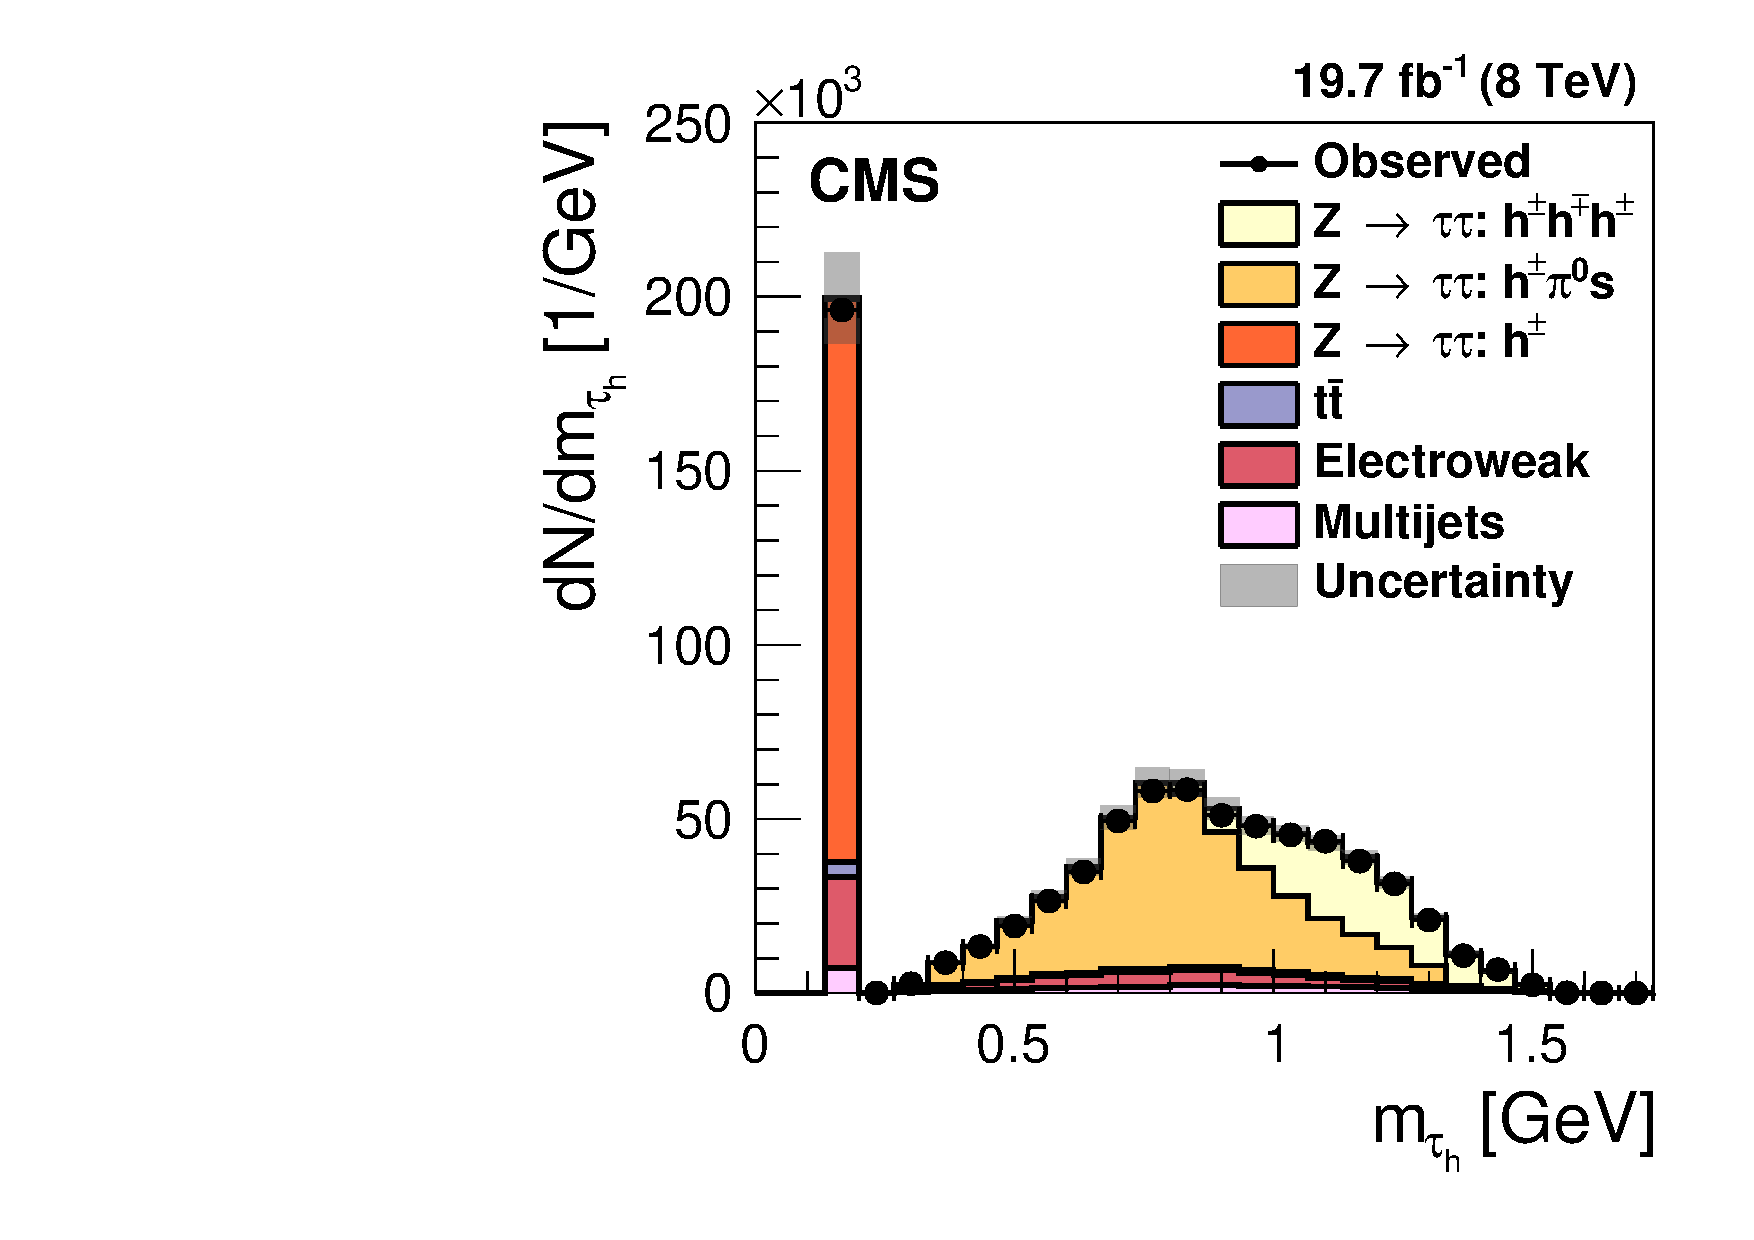
\includegraphics[width=0.55\textwidth]{object_reconstruction_and_selection/plots/CMS-TAU-14-001_tau_mass.pdf}
     \caption{
The reconstructed invariant mass of the $\tauh$ candidate. A spike is seen at 140\MeV for the 1-prong
$\tauh$ decay mode where the mass is assigned equal to the mass of a $\pi^{\pm}$. The 1-prong+$\PGpz$
decay mode is seen to peak around 770\MeV while the 3-prong decay mode centers around 1260\MeV.
     }
     \label{fig:tau_mass}
\end{figure*}

The dynamic strip reconstruction has been optimized to best reconstruct the $\PGpz$ 
decay products. It was found that the fixed width strips used in Run-I
occasionally allowed the $\PGpz$ decay products to escape the boundaries of the strip and would result in
the escaped particle being added to the isolation sums for the $\tauh$ and not contributing
to the energy or momentum of the $\tauh$. Widening the fixed width strips can be used to catch
these escaping particles. However, considering that more boosted $\tauh$ will have a more 
collimated structure, it is also helpful to narrow the strip at higher $\tauh$ $\pt$ to suppress
pileup or other non-$\tau$ contributions when possible. The strip widths are calibrated to
on simulations that target retaining 95\% of the $\PGpz$ decay products, see Figure~\ref{fig:tau_dyn_strip}.
Strips containing one or more electron of photon constituent and passing a cut of $\pt > 2.5\GeV$
for the sum of the electrons and photons are kept as $\PGpz$ candidates. 

\begin{figure*}[htbp]
\centering
     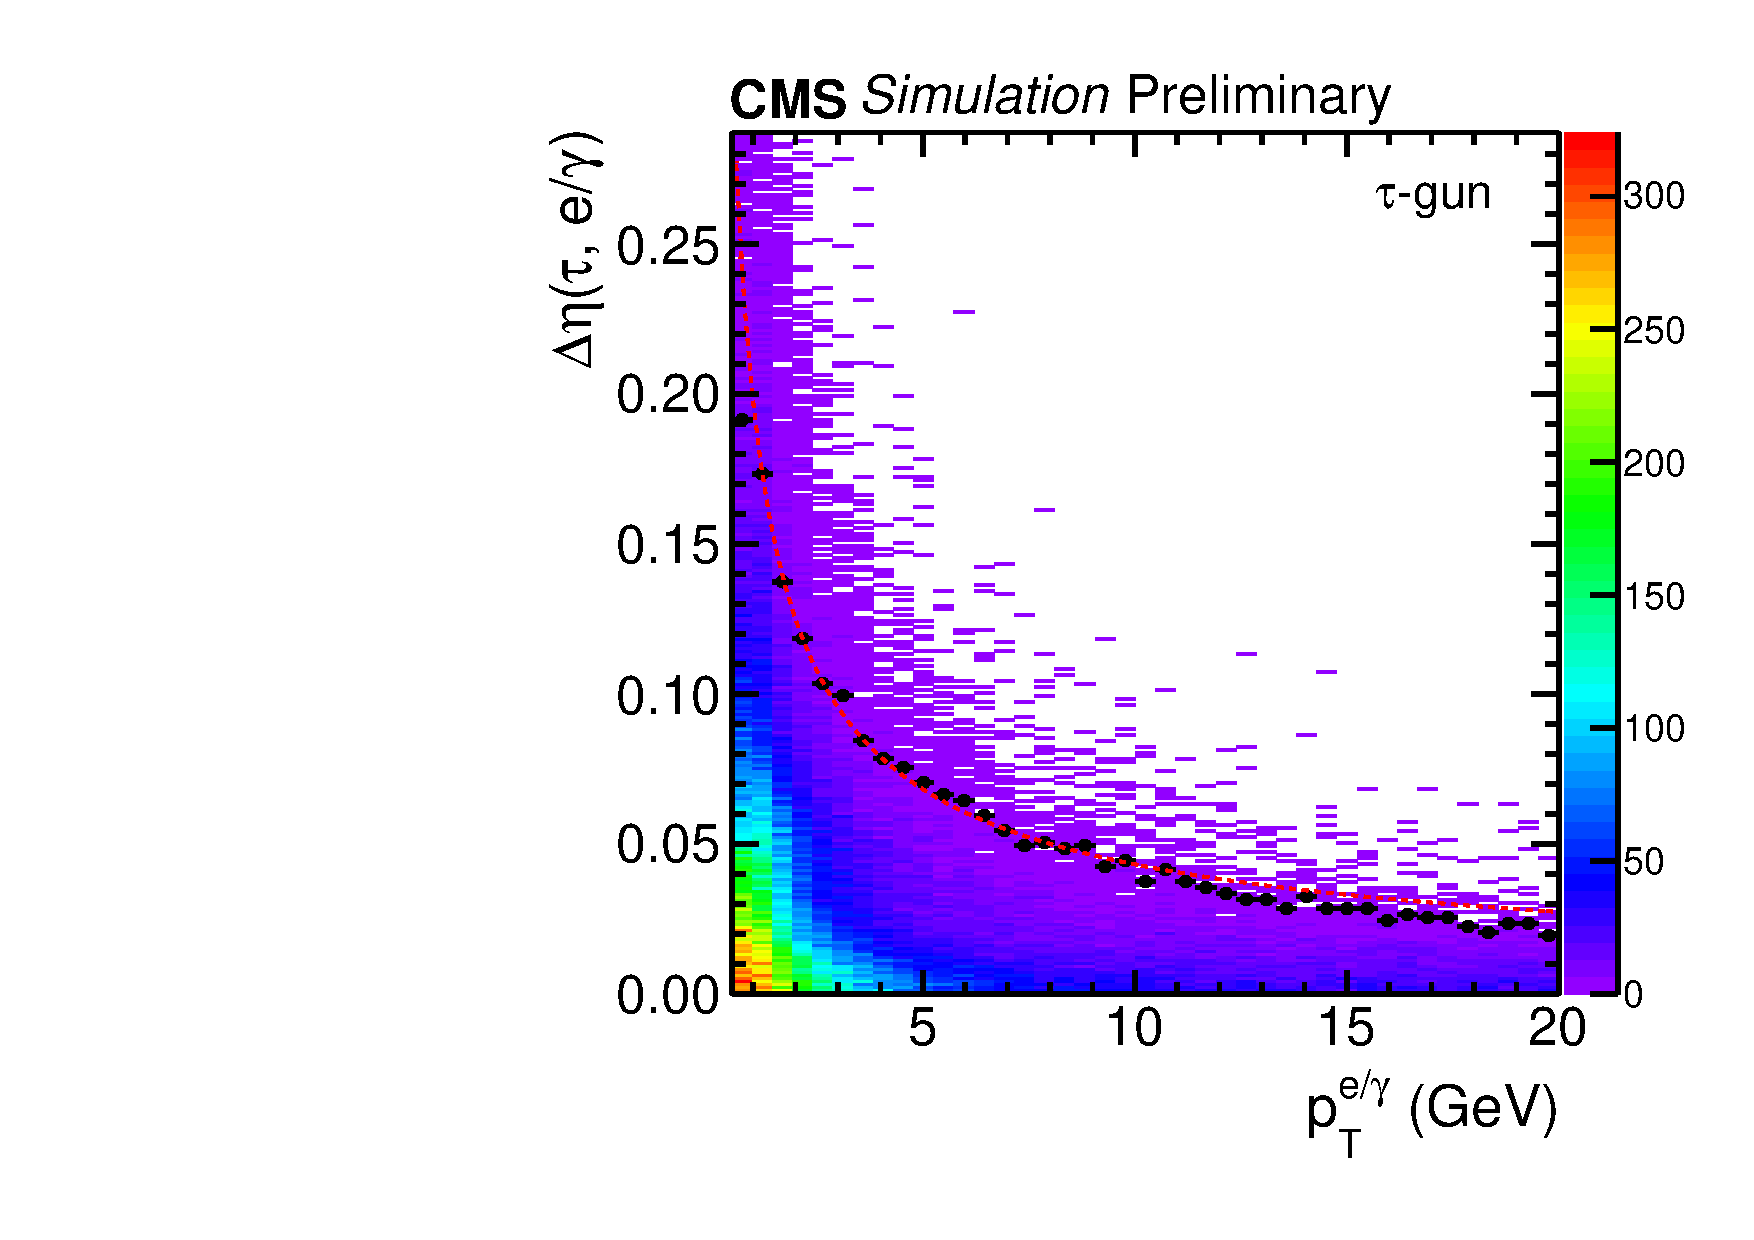
\includegraphics[width=0.45\textwidth]{object_reconstruction_and_selection/plots/tau_dyn_strip_eta.pdf}
     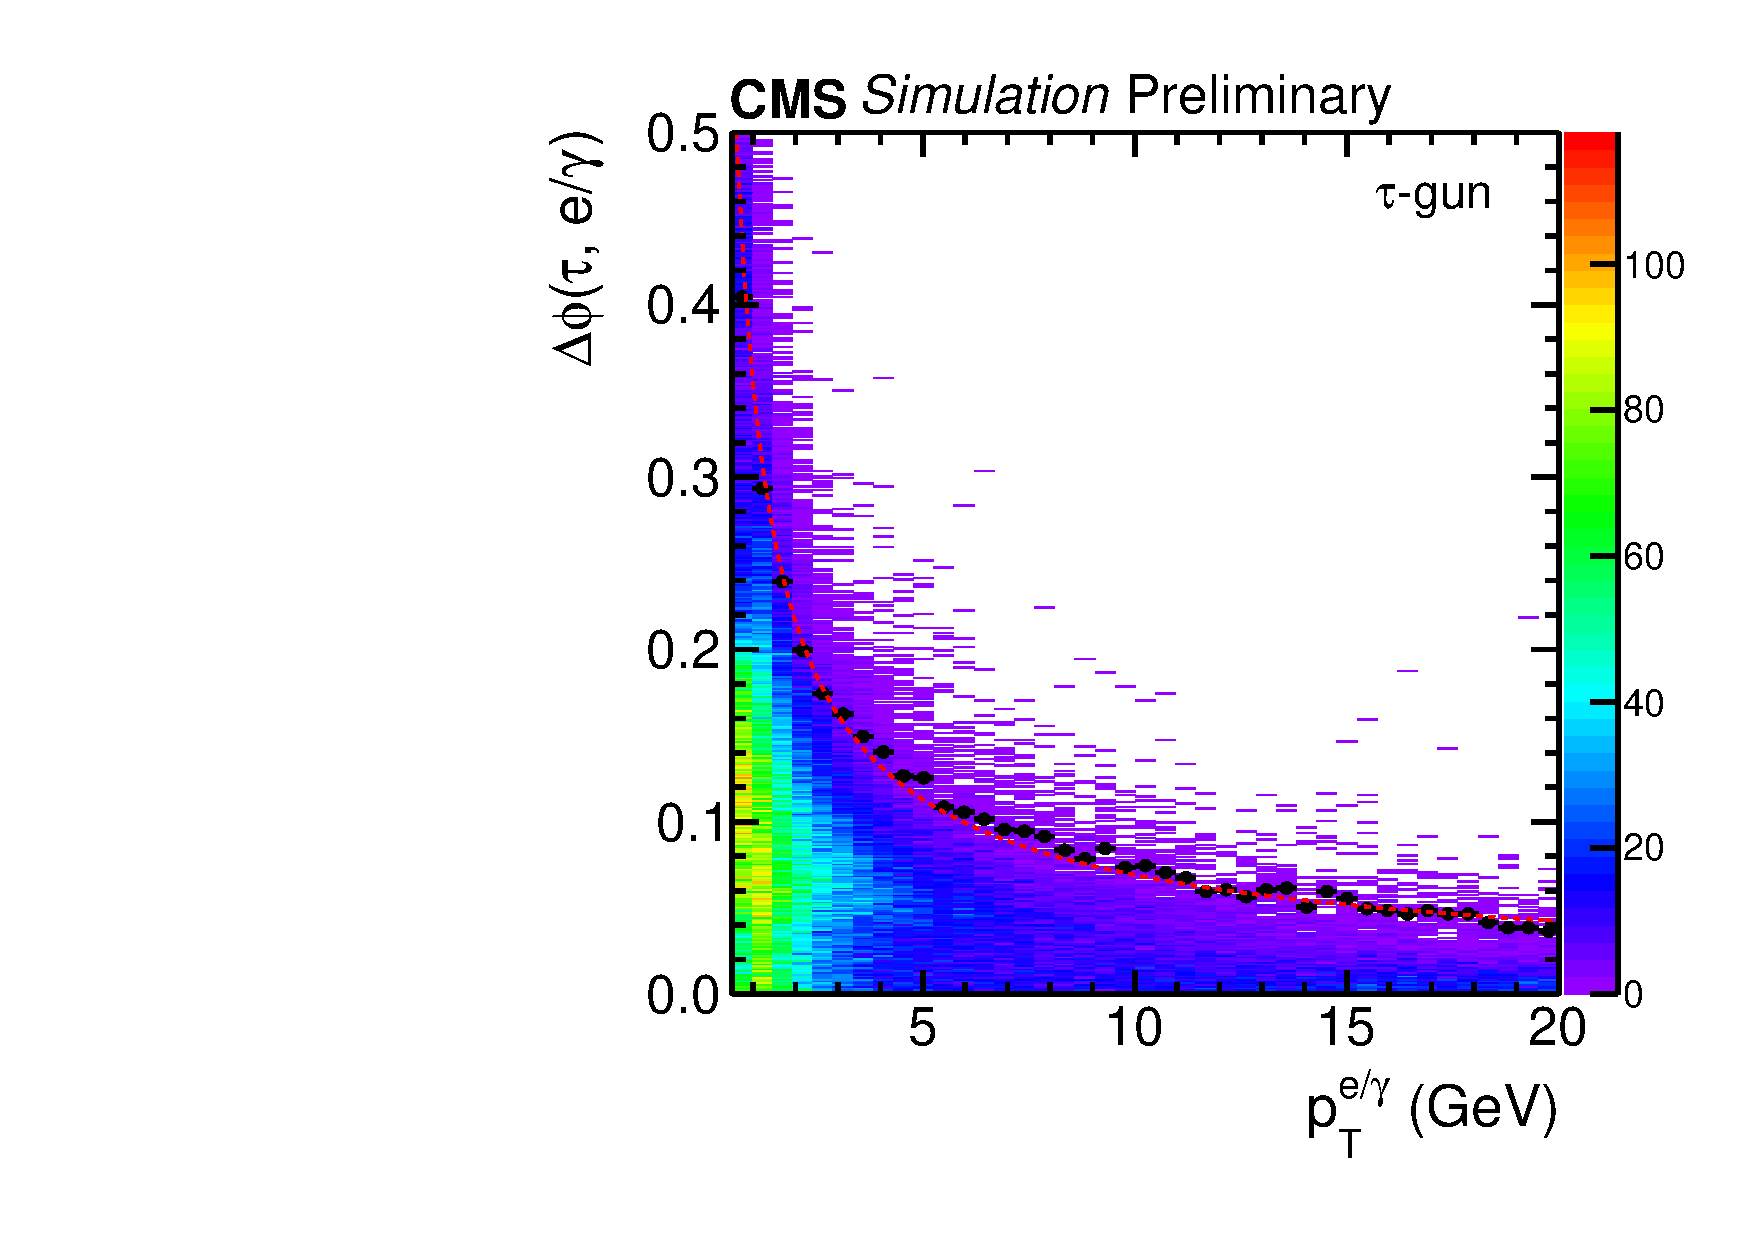
\includegraphics[width=0.45\textwidth]{object_reconstruction_and_selection/plots/tau_dyn_strip_phi.pdf}
     \caption{
Distance in $\eta$ (left) and $\phi$ (right) between $\tauh$ and e/$\gamma$, that are due to 
hadronic tau decay
products, as a function of e/$\gamma$ $\pt$. The size of the window is larger in the $\phi$
direction due to bending in the magnetic field. The dotted line shows the 95\%
quantile while the red line shows the fit to the 95\% quantile. The red line is used
to define the widths of the dynamic strip.
     }
     \label{fig:tau_dyn_strip}
\end{figure*}

A multivariate (MVA) discriminator~\cite{Hocker:2007ht}, including isolation, shape-based variables
and lifetime information, is used to reduce the rate for  quark and gluon initiated jets
to be identified as $\tauh$ candidates. The working point used in the $\htt$ analysis, \texttt{Tight Tau MVA},
has an efficiency of about 60\% for genuine $\tauh$,
with about 1\% misidentification rate for quark- and gluon-initiated jets, for a $\pt$ range typical 
of $\tauh$ originating from a $\PZ$ boson. A looser working point is used in the Higgs associated 
production analysis ZH final states, \texttt{Medium Tau MVA}, which as an efficiency of 65\% for genuine
$\tauh$ with a 2\% misidentification rate.

Electrons and muons can both be reconstructed as $\tauh$ candidates, usually into the 1-prong or
1-prong+$\PGpz$ decay modes. For electrons this can happen easily when an electron emits a bremsstrahlung
photon mimicking a $\PGpz$s in the decay mode reconstruction. MVA discriminants have been developed 
which specifically target the suppression of electrons and muons being misidentified as 
$\tauh$~\cite{Khachatryan:2015dfa, CMS-PAS-TAU-16-002}.
A range of anti-e and anti-$\Pgm$ discriminant working points are used in these analyses. The choice
of which working point to use is tailored towards suppressing the dominant backgrounds in different
final states and is discussed in detail in the analysis sections~\ref{sec:htt_analysis, sec:vh_analysis}.


